\documentclass[10pt, conference]{IEEEtran}
%Enabled blocked functionality
\IEEEoverridecommandlockouts
%Define custom IEEEpubid that will place it self in a column and not a page, suitable from conference class
% \IEEEpubid{\makebox[\columnwidth]{978-1-5386-9111-3/19/\$31.00 \copyright2019 IEEE \hfill} \hspace{\columnsep}\makebox[\columnwidth]{  }}
% The preceding line is only needed to identify funding in the first footnote. If that is unneeded, please comment it out.
\usepackage{cite}
\usepackage{multirow}
\usepackage{amsmath,amssymb,amsfonts}
\usepackage{algorithmic}
\usepackage{graphicx}
\usepackage{textcomp}
\usepackage{times}
\usepackage{tabularx}
\usepackage{subfiles}
\usepackage{amsmath}
\usepackage{amsfonts}
\usepackage{amssymb}
\usepackage{graphicx}
\usepackage{array}
\usepackage[bookmarks=false]{hyperref}
\usepackage{float}
\usepackage{url}
\usepackage{listings}
\usepackage{wrapfig}
%\usepackage{caption}
\usepackage{cite}
\usepackage{tabularx}
\usepackage{times}
\usepackage{algorithmic}
\usepackage{algorithm}
\usepackage{tikz}
\usetikzlibrary{shapes,arrows}
\usepackage{pgfplots}
\usepackage{arydshln}
\usepackage{rotating}
%\usepackage{adjustbox}
\def\BibTeX{{\rm B\kern-.05em{\sc i\kern-.025em b}\kern-.08em
		T\kern-.1667em\lower.7ex\hbox{E}\kern-.125emX}}

% Define block styles
\tikzstyle{decision} = [diamond, draw, fill=blue!20, 
text width=4.5em, text badly centered, node distance=3cm, inner sep=0pt]
\tikzstyle{block} = [rectangle, draw, fill=blue!20, 
text width=24em, text justified, rounded corners, minimum height=4em]
\tikzstyle{block1} = [rectangle, draw, fill=green!20, 
text width=15em, text justified, rounded corners, minimum height=3em]
\tikzstyle{line} = [draw, -latex']
\tikzstyle{cloud} = [draw, ellipse,fill=red!20, node distance=3cm,
minimum height=2em]

\usepackage{eso-pic}
\newcommand\AtPageUpperMyright[1]{\AtPageUpperLeft{%
		\put(\LenToUnit{0.08\paperwidth},\LenToUnit{-1cm}){%
			\parbox{\textwidth}{\raggedleft\fontsize{10}{11}\selectfont #1}}%
}}%
\newcommand{\conf}[1]{%
	\AddToShipoutPictureBG*{%
		\AtPageUpperMyright{#1}
	}
}
\begin{document}
	
	\title{Statistical Approach for Classifying Sentiment Reviews by Reducing Dimension using Truncated Singular Value Decomposition
	}
	\author{
		\IEEEauthorblockN{
			Asmaul Husna
			}
			\IEEEauthorblockA{
				\textit{Department of Information Technology} \\
				\textit{University of Information Technology \& Sciences}\\
				Dhaka, Bangladesh \\
				asmaul.husna@uits.edu.bd}
		\and
		\IEEEauthorblockN{
			Habibur Rahman
		}
		\IEEEauthorblockA{
			\textit{Department of Computer Science \& Engineering} \\
			\textit{Rajshahi University of Engineering \& Technology }\\
			Rajshahi, Bangladesh \\
			habib\_cse\_ruet@yahoo.com
		}
		\and
		\IEEEauthorblockN{
		    \hspace{13em} Emrana Kabir Hashi
		}
		\IEEEauthorblockA{
			 \hspace{15em}\textit{Department of Computer Science \& Engineering} \\
			 \hspace{15em}\textit{Rajshahi University of Engineering \& Technology }\\
			 \hspace{15em}Rajshahi, Bangladesh \\
			 \hspace{15em}emrana.kabir@ruet.ac.bd
		}
	}
	\maketitle
% 	\IEEEpubidadjcol
% 	\conf{1st International Conference on Advances in Science, Engineering and Robotics Technology (ICASERT-2019), May 3--5, 2019}

	\begin{abstract} Human sentiments, the attitudes, thoughts, or the judgments backed by feelings are the most important factors for the field of science and business which can be expressed through the web. The rapid growth of unstructured sentiment data has created a very big challenge to provide a fast and cost-efficient model for sentiment analysis.  The aim of this paper is to find positive and negative emotions from the public comments rapidly and effectively. In this paper,  to vectorize the text reviews and to reduce the dimension of the vectorized data, Term Frequency-Inverse Document Frequency (TF-IDF) and Truncated Singular Value Decomposition (TSVD) is used respectively. An efficient approach has been provided using the logistic regression algorithm employed in a vector space model of affective knowledge which gives fast learning speed. In result, this proposed method has reduced the learning time by 42.63\% with the reduction of dimension from 12209 to 100 and has reported almost the same accuracy which is 85.7\%  and 89.3\% for the movie review and yelp restaurant review dataset respectively. In comparison to existing methods, this method has shown almost the same accuracy after dimension reduction. Our result showed that our proposed system is useful.
	\end{abstract}
	
	\begin{IEEEkeywords}
		Sentiment Analysis, Logistic Regression, Truncated Singular Value Decomposition, Vector Space Model
	\end{IEEEkeywords}
	\section{Introduction}
	In this modern era, people are very much dependent on social networks, blogs and other online media for expressing their opinions and sentiments. The availability of these web communities gives opportunity to people for sharing their opinions and ideas in a cost and time efficient way. This huge source of information and opinions has provided a powerful communication medium to share knowledge and to get advantage from others’ experience. At present, it is a key factor for the organizer to distill the knowledge from unstructured web data of public opinions and identify the mind of the customers about their products, policies, and organizations.
	
	Sentiment analysis is a process of extracting positive and negative opinions from the review of people about anything. But the review of people which means the unstructured web data is hardly accessible to computers and for this, extraction the reviews into positive and negative is difficult. For solving this problem, a different type of machine learning algorithm exists. Such algorithms are very good at retrieving text, splitting them into parts, counting their words and finally giving a positive or negative result \cite{b1, b2}. Most of the researchers have only focused on which algorithm is superior to others for extracting reviews but they have not considered time and cost \cite{b10 , b11, b12, b13, b14, b15, b16}. But as the amount of social data is increasing rapidly, time and cost is also a big issue for sentiment analysis.

	In this paper, we have focused on not only extracting positive and negative reviews but also the optimal use of time, storage space, and cost. There are several types of feature extraction method and dimension reduction technique. Among them, Term Frequency-Inverse Document Frequency(TF-IDF) and Truncated Singular Value Decomposition(TSVD) have been used for feature extraction and dimension reduction respectively which perform the main role in reducing time and cost. Logistic regression has been used as a machine learning algorithm for extracting sentiment for its fast learning speed. Present related works and their limitations, our proposed framework, evaluation the performance have been described in the next sections subsequently. Finally, we have concluded our research with future work.
	
	\section{Related Works}
	Sentiment analysis is one of the recent hot topics for social, political, scientific and business world. Sentiment analysis depends on the natural language texts. Natural language texts are using in a wide range from questions and answering to mathematical word problem solving \cite{b3}. For classify the sentiments, Support Vector Machine (SVM) \cite{b4, b5, b6}, Naïve Bayes (NB) \cite{b7, b8} and Maximum Entropy (ME) \cite{b9, b10} are the most popular machine learning algorithms.
	
	In paper \cite{b11}, 82.9\% accuracy has been got for movie reviews using SVM with a bag of words feature sets. Naïve Bayes, ME have also been used but SVM is superior among them. In paper \cite{b12}, they have trimmed out objective content from movie reviews and used SVM and NB bag of words classifier to determine review polarity with an accuracy of 87.15\%. They have examined the relation between subjectivity detection and polarity classification. For subjectivity detection, a graph has been built where source and sink corresponded to the class of subjective and objective sentences, respectively. Semi-supervised learning for imbalanced sentiment classification has been addressed in \cite{b13}. They have only focused on the imbalanced problem in the initial labeled data.
	
	A novel approach using SVM to find out the overall positive and negative scores for a particular feature has presented in \cite{b14}. SVM has been showed as a best than other machine learning algorithm. In paper \cite{b15}, Delta TF-IDF has been introduced for subjectivity detection and sentiment polarity classification, as well as documents of varying sizes. They have shown their improved result using SVM. Different corpora available for scientific research in opinion mining have been compared in \cite{b16}. They have applied machine learning algorithm (SVM) for different corpora.
	
	For aspect-based sentiment analysis in \cite{b17}, SVM and Logistic Regression \cite{b21} have been used as supervised machine learning algorithm. But they analyzed their result only for higher dimension. After analyzing above papers, we can see that in most paper researchers used SVM as a machine learning algorithm for sentiment mining. But in this paper, we have used logistic regression algorithm and compared with SVM using dimension reduction technique.
	
	\section{Proposed System}
The goal of our system is to analysis sentiment with cost-effective way. Fig. \ref{fig:flow} gives the overview of our proposed system.

\begin{figure}[H]
    \begin{center}
        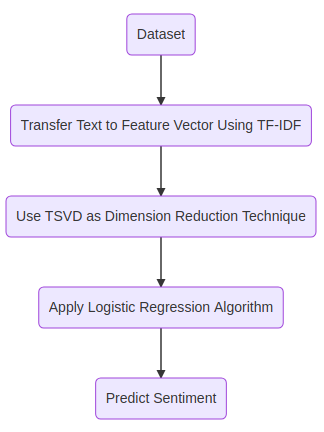
\includegraphics[width = 0.191 \textheight]{flow.png}
    \end{center}
	\caption{Flow of the proposed system}
	\label{fig:flow}
\end{figure}
	
	In the following sections, we discussed the detailed methodology:
	
	\subsection{\textbf{Dataset:}} We have used the movie review dataset and the yelp restaurant review dataset \cite{b24}. Movie review dataset is derived from the benchmark corpus developed by Pang and Lee \cite{b18}. Those corpus includes 1000 positive and 1000 negative movie reviews. We have divided the datasets into train set and test set using 10 fold cross-validation.
	
	\subsection{\textbf{Text to Feature Vector: }} Vector space model represents the text documents as vectors of identifiers. It is used in information filtering, information retrieval etc. Term Frequency-Inverse Document Frequency (TF-IDF) \cite{b20} is one of the examples of vector space model. It is used for transforming text to feature vector. Actually, TF-IDF is a numerical statistics that determines how important a word is in a corpus. As 83\% of text-based recommended systems in the domain of digital libraries use TF-IDF, we have selected it.
	
	Suppose, we have a set of English text document. The term frequency of a term(word) in this document is proportional to the number of occurrence of the term in this document. So it can be defined as $tf(t,d) = F(t,d)$ where $F(t,d)$ is number of occurrences of term, $t$ in document, $d$. Inverse document frequency diminishes the weight of terms that occur very frequently in the document set and increases the weight of terms that occur rarely. It is defined as the \eqref{eq:idf}:
	\begin{equation}
	idf(t, D) = \log \dfrac{N} {N_{t\in D}}
	\label{eq:idf}
	\end{equation}
	Here, $N$ is the total number of files in the corpus $D$ and $N_{t\in d}$ is the number of files in which term, $t$ is present. Finally, \textit{tf-idf} is calculated as the following \eqref{eq:tfidf}:
	\begin{equation}
		tf-idf(t, d, D) = tf(t, d) \times idf(t, D)
		\label{eq:tfidf}
	\end{equation}
	
	\subsection{\textbf{Dimension Reduction:}}
	Truncated Singular Value Decomposition (TSVD) reduces the time and storage space by converting higher dimension into the lower dimension \cite{b23}. By removing multi-collinearity, it improves the performance of machine learning algorithm. We have selected 100 as the lower dimension. TSVD is preferred to other dimension reduction technique for its simplicity and relatively low computational cost. It is particularly suitable for measuring cross-correlations between affective word or concept.
	
	\subsection{\textbf{Logistic Regression Algorithm:}} Logistic Regression has proven highly effective in natural language processing and text classification \cite{b20, b21}. It was developed by David Cox in 1958 \cite{b22}.
	
	We have chosen the approach in \cite{b20} for Logistic Regression algorithm cause this approach simultaneously avoids overfitting and maintains high learning speed. It is also appropriate when the dependent variable is binary. As we require a binary efficient classifier, we have chosen it. Besides this, it works by maximizing posterior class probability. So, for the lower dimension, it works efficiently in terms of time and accuracy.
	
	Logistic regression measures the relationship between the categorical dependent variable and one or more independent variables by estimating probabilities using a logistic function.
	
	\begin{figure}[H]
		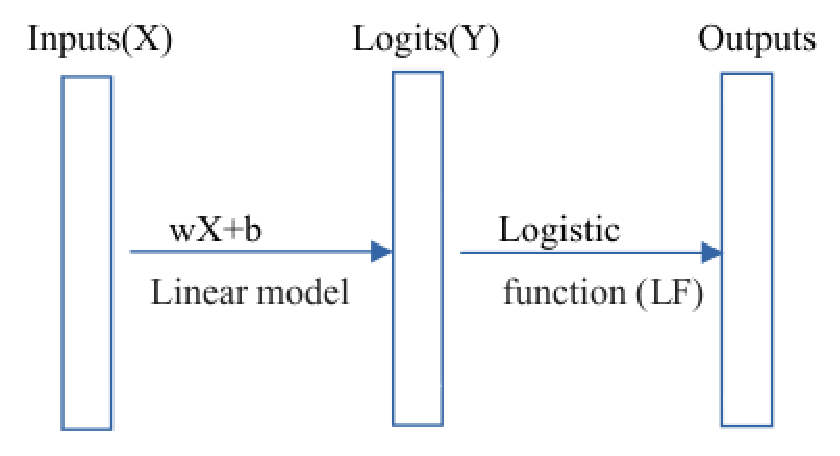
\includegraphics[width = 0.35\textheight]{logisticRegression}
		\caption{Model of Logistic Regression Algorithm}
		\label{fig:train}
	\end{figure}
	where, weight of the corresponding input, $w$ and bias input, $b$ and \textit{LF} represents Logistic Function as follow \eqref{eq:lf}:
	\begin{equation}
		LF = \dfrac{e_y}{1 + e_y}
		\label{eq:lf}
	\end{equation}
	
	\section{Performance evaluation}
	
	For sentiment analysis using machine learning algorithm most of the existing system have used SVM and they have proved that SVM is superior to others. But most of them have not used any dimension reduction technique and have not considered time, dimension and cost. So, we have compared our system with SVM with dimension reduction technique. Time has also been considered in this performance evaluation. Finally, we have compared our result with the results of the existing systems.
	
	\subsection{\textbf{Hardware and Software Configuration:}}
	\begin{itemize}
		\item \textbf{Operating System:} Linux
		\item \textbf{Programming Language:} Python 2.7
		\item \textbf{Processor:} Intel Core i5-3317U CPU @ 1.70GHz 
		\item \textbf{RAM:} 4GB
	\end{itemize}
	
	\subsection{\textbf{Result Analysis and Comparison:}} Dimension of the training data has been evaluated before using TSVD. Then 10 fold cross-validation has been used. We have got the following result from Logistic Regression and SVM. We have also shown the confusion matrix for both algorithms in \ref{table:comp}. 
	
		\begin{table}[H]
		\caption{Confusion Matrix Without Dimension Reduction}
		\begin{center}
% 		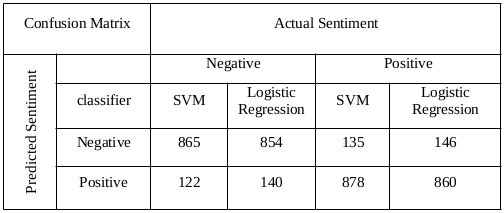
\includegraphics[width = 0.35\textheight]{table1.png}
% 			\hspace{0.1cm}
			\begin{tabular}{|*{6}{c|}}
			    \hline
			    \multicolumn{6}{|c|}{\textbf{Movie Review Dataset}}\\
				\hline
				\multicolumn{2}{|c|}{\textbf{}} & \multicolumn{4}{|c|}{\textbf{Actual}}\\
				\hline
				\multirow{4}{*}{\begin{sideways}\textbf{Predicted}\end{sideways}} & & \multicolumn{2}{|c|}{\textbf{Neg.}} & \multicolumn{2}{|c|}{\textbf{Pos.}}\\
				\cline{2-6}
				& \textbf{Classifier} & \textbf{SVM} & \textbf{LR} & \textbf{SVM} & \textbf{LR}\\  \cline{2-6}
				& \textbf{False} & 850 & 864 & 150 & 136\\
				\cline{2-6}
				& \textbf{True} & 154 & 137 & 846 & 863\\
				\hline
				\hline
			    \multicolumn{6}{|c|}{\textbf{Yelp Restaurant Review Dataset}}\\
				\hline
				\multicolumn{2}{|c|}{\textbf{}} & \multicolumn{4}{|c|}{\textbf{Actual}}\\
				\hline
				\multirow{4}{*}{\begin{sideways}\textbf{Predicted}\end{sideways}} & & \multicolumn{2}{|c|}{\textbf{Neg.}} & \multicolumn{2}{|c|}{\textbf{Pos.}}\\
				\cline{2-6}
				& \textbf{Classifier} & \textbf{SVM} & \textbf{LR} & \textbf{SVM} & \textbf{LR}\\  \cline{2-6}
				& \textbf{False} & 907 & 907 & 93 & 93\\
				\cline{2-6}
				& \textbf{True} & 117 & 106 & 883 & 894\\
				\hline
			\end{tabular}
			\label{table:comp}
		\end{center}
	\end{table}
	From confusion matrix, we can measure the accuracy like the \eqref{eq:acc}.
	\begin{equation}
	    Accuracy = \dfrac{T_p + T_n}{T_p + T_n + F_p + F_n}
	    \label{eq:acc}
	\end{equation}
	where, $T_p = $True Positive, $T_n = $ True Negative, $F_p = $ False Positive, and $F_n = $ False Negative.
	
	\begin{table}[H]
		\caption{Result Analysis without Dimension reduction}
		\begin{center}
		\begin{tabular}{|*{4}{c|}}
        \hline
        \multicolumn{4}{|c|}{Movie Review Dataset}\\
        \hline
        \textbf{Classifier} & \textbf{Accuracy(\%)} & \textbf{\#Features} & \textbf{Training Time}\\
        \hline
        \textbf{SVM} & 84.8 & 12209 & 8.1166726\\
        \hline
        \textbf{LR} & \textbf{86.35} & 12209 & \textbf{0.0763286}\\
        \hline
        \multicolumn{4}{|c|}{Yelp Restaurant Review Dataset}\\
        \hline
         \textbf{Classifier} & \textbf{Accuracy(\%)} & \textbf{\#Features} & \textbf{Training Time}\\
        \hline
        \textbf{SVM} & 89.5 & 12209 & 1.4578088\\
        \hline
        \textbf{LR} & \textbf{90.05} & 12209 & \textbf{0.069607299}\\
        \hline
        \end{tabular}
% 		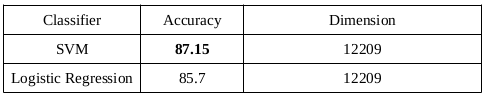
\includegraphics[width = 0.35\textheight]{table2.png}
			\label{table:rwodr}
		\end{center}
	\end{table}
	
	After the dimension reduction, we have shown the fixed dimension and the training time for both algorithms in the following table \ref{table:cmdr}.
	
	\begin{table}[H]
		\caption{Confusion Matrix after Dimension Reduction}
		\begin{center}
		\begin{tabular}{|*{6}{c|}}
			    \hline
			    \multicolumn{6}{|c|}{\textbf{Movie Review Dataset}}\\
				\hline
				\multicolumn{2}{|c|}{\textbf{}} & \multicolumn{4}{|c|}{\textbf{Actual}}\\
				\hline
				\multirow{4}{*}{\begin{sideways}\textbf{Predicted}\end{sideways}} & & \multicolumn{2}{|c|}{\textbf{Neg.}} & \multicolumn{2}{|c|}{\textbf{Pos.}}\\
				\cline{2-6}
				& \textbf{Classifier} & \textbf{SVM} & \textbf{LR} & \textbf{SVM} & \textbf{LR}\\  \cline{2-6}
				& \textbf{False} & 818 & 849 & 182 & 151\\
				\cline{2-6}
				& \textbf{True} & 208 & 135 & 792 & 865\\
				\hline
				\hline
			    \multicolumn{6}{|c|}{\textbf{Yelp Restaurant Review Dataset}}\\
				\hline
				\multicolumn{2}{|c|}{\textbf{}} & \multicolumn{4}{|c|}{\textbf{Actual}}\\
				\hline
				\multirow{4}{*}{\begin{sideways}\textbf{Predicted}\end{sideways}} & & \multicolumn{2}{|c|}{\textbf{Neg.}} & \multicolumn{2}{|c|}{\textbf{Pos.}}\\
				\cline{2-6}
				& \textbf{Classifier} & \textbf{SVM} & \textbf{LR} & \textbf{SVM} & \textbf{LR}\\  \cline{2-6}
				& \textbf{False} & 846 & 901 & 154 & 99\\
				\cline{2-6}
				& \textbf{True} & 103 & 115 & 897 & 885\\
				\hline
			\end{tabular}
% 		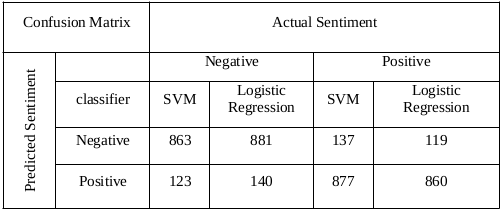
\includegraphics[width = 0.35\textheight]{table3.png}
			\label{table:cmdr}
		\end{center}
	\end{table}
	
	\begin{table}[H]
		\caption{Result Analysis after Dimension Reduction}
		\begin{center}
        \begin{tabular}{|*{4}{c|}}
        \hline
        \multicolumn{4}{|c|}{Movie Review Dataset}\\
        \hline
        \textbf{Classifier} & \textbf{Accuracy(\%)} & \textbf{\#Features} & \textbf{Training Time}\\
        \hline
        \textbf{SVM} & 80.5 & 100 & 0.5638779\\
        \hline
        \textbf{LR} & \textbf{85.7} & 100 & \textbf{0.0437935}\\
        \hline
        \multicolumn{4}{|c|}{Yelp Restaurant Review Dataset}\\
        \hline
         \textbf{Classifier} & \textbf{Accuracy(\%)} & \textbf{\#Features} & \textbf{Training Time}\\
        \hline
        \textbf{SVM} & 88.65 & 100 & 0.5866717\\
        \hline
        \textbf{LR} & \textbf{89.3} & 100 & \textbf{0.0398641}\\
        \hline
        \end{tabular}
% 		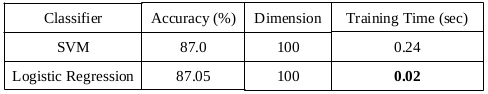
\includegraphics[width = 0.35\textheight]{table4.png}
		\label{table:radr}
		\end{center}
	\end{table}
	Now comparing Table II and Table IV, we can see that accuracy of Table IV slightly decreases. But in terms of dimension and training time, Table IV is superior.	When SVM has been used without reducing dimension, it is better than Logistic Regression in terms of accuracy. But when dimension has been reduced, Logistic Regression is better than SVM.
	
	Fig. \ref{fig:compM} shows the comparison of training time before and after the dimension reduction for SVM and LR.
	\begin{figure}[H]
		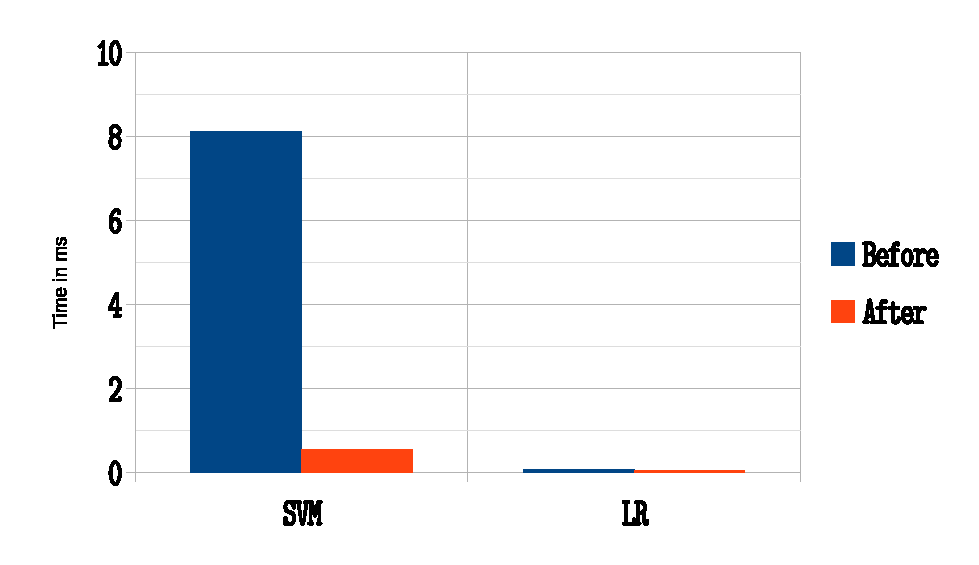
\includegraphics[width = 0.35\textheight]{trainingTime.eps}
		\caption{Comparison of Training Time}
		\label{fig:compM}
	\end{figure}
	
	Dimension of movie review data has been decreased from 12209 to 100 using TSVD. For this, storage space and cost both have been decreased. Besides this, from table IV we can see that Logistic Regression is 42.63\% fast according to training time but the accuracy is almost same.
	
	In terms of the number of features, our proposed system uses 100 features which is reduced by TSVD. On the otherhand, previous two methods \cite{b11, b14} have not used any dimension reduction techniques. Fig. \ref{fig:fea} shows the comparison of features.
	
	\begin{figure}[H]
		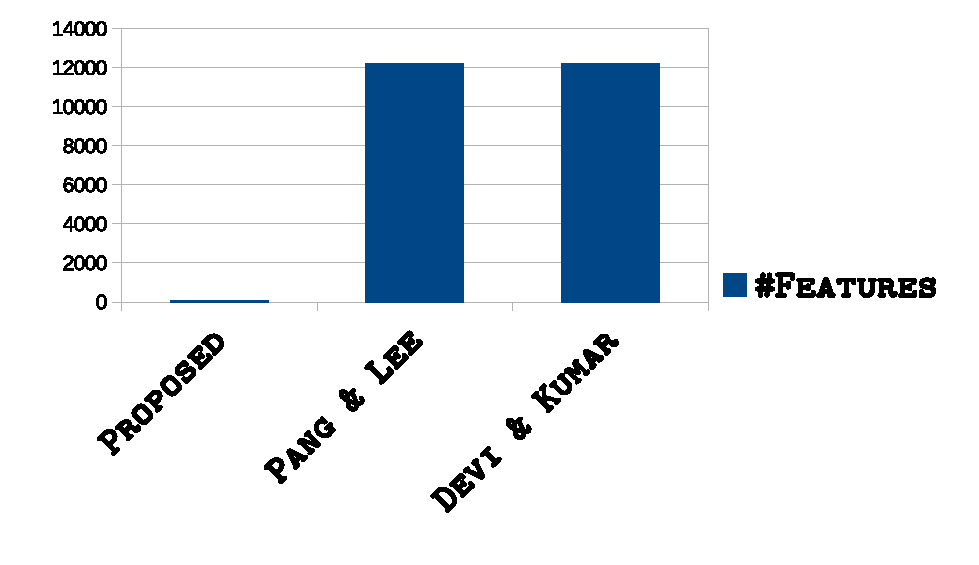
\includegraphics[width = 0.35\textheight]{features.eps}	\caption{Comparison of Features}
		\label{fig:fea}
	\end{figure}
	
	For movie review dataset, our proposed systems shows an accuracy of 85.7\% while \cite{b11} was 82.9\%. Compared to \cite{b11}, our system is superior. But \cite{b14} was 90.85\% accurate which is superior to our system and \cite{b11}. Fig. \ref{fig:acc} depicts the comparison:
    \begin{figure}[H]
    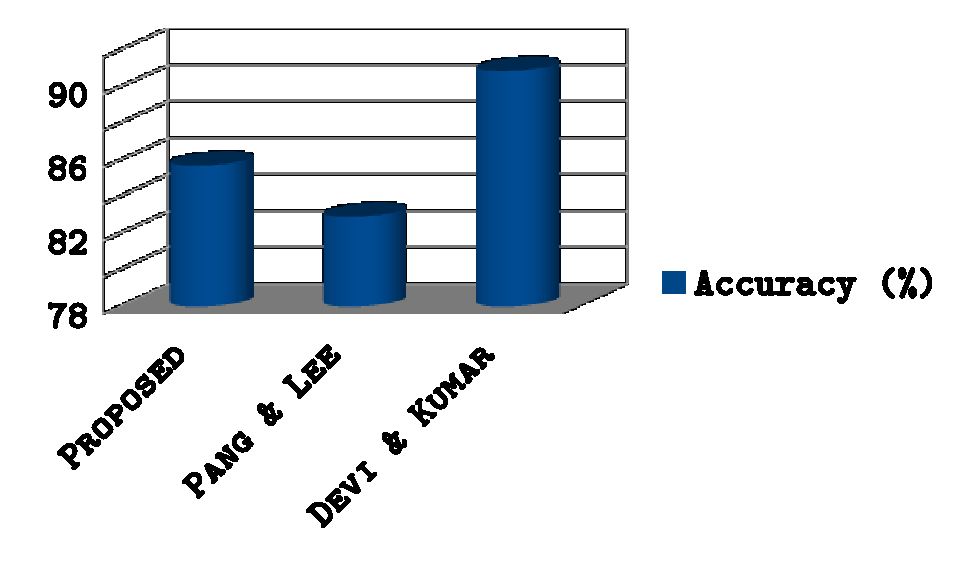
\includegraphics[width = 0.35\textheight]{acc.eps}
    \caption{Comparison of Accuracy}
    \label{fig:acc}
    \end{figure}
	
	In conclusion, our proposed system is more accurate than \cite{b11} and \cite{b14} for movie review dataset in terms of features.
	
	\section{Conclusion and Future Work} The main goal of this paper is to introduce a new framework for sentiment analysis which is both time and cost efficient by dimension reduction. The dimension also increases for sentiment analysis from large-scale data. For this learning time of any algorithm increases which is an important factor for measurement performance of any system. The system with faster speed and reasonable accuracy are more appropriate for sentiment analysis than the slower system with high accuracy. By analyzing above result, we can come to a conclusion that the accuracy of our system is almost same to the system using SVM after using dimension reduction technique. But in terms of training time, Logistic Regression is better than SVM. Besides this, the dimension of the proposed system is comparably very low. So our system is cost-effective and we have successfully provided a time and cost efficient model for sentiment analysis.
	
	Unigram TF-IDF has been used for transforming text to feature vector. Bigram TF-IDF and deep learning can be used in future for more accurate result.
	
	\section*{Acknowledgments}The authors of this paper are grateful to all the members of the Syntax and Semantic Research Group, Bangladesh. Authors are also thankful to the Rajshahi University of Engineering and Technology, and to the University of Information Technology and Sciences.
	
	\begin{thebibliography}{00}
		\bibitem{b1} B. Pang and L. Lee, ``Opinion mining and sentiment analysis," Foundations and Trends in Information Retrieval, vol. 2, pp. 1-135, January 2008.
		
		\bibitem{b2} B. Liu, ``Sentiment analysis and opinion mining," Morgan and Claypool, April 2012.
		
		\bibitem{b3} Habibur Rahman, Julia Rahman, and Asmaul Husna, ``WALGES: Weighted Probability Based Scoring Approach for Solving Algebraic Word Problems using Semantic Parsing", in Proc. of the International Conference on Electrical, Computer and Communication Engineering, February 2019.
		
		\bibitem{b4} T. Joachims, ``Text Categorization with Suport Vector Machines: Learning with Many Relevant Features," in Proceedings of the 10th European Conference on Machine Learning, April 1998,  pp. 137-142.
		
		\bibitem{b5} T. Joachims, ``Making large-scale support vector machine learning practical," MIT Press Cambridge, MA, USA , 1999.
		
		\bibitem{b6} E. Leopold and J. Kindermann,``Text Categorization with Support Vector Machines. How to Represent Texts in Input Space?," Machine Learning, vol. 46, pp. 423-444, March 2002.
		
		\bibitem{b7} D. D. Lewis, ``Naive (Bayes) at Forty: The Independence Assumption in Information Retrieval," in Proceedings of the 10th European Conference on Machine Learning, April 1998, pp. 4-15.
		
		\bibitem{b8} S. B. Kim, K. S. Han, H. C. Rim and S. H. Myaeng, ``Some Effective Techniques for Naive Bayes Text Classification," IEEE Transactions on Knowledge and Data Engineering, vol. 18, pp. 1457-1466, November  2006.
		
		\bibitem{b9} A. L. Berger, V. J. D. Pietra and S. A. D. Pietra,``A maximum entropy approach to natural language processing," Computational Linguistics, vol. 22, pp. 39-71, March 1996.
		
		\bibitem{b10} K. Nigam, J. Lafferty and A. McCallum, ``Using maximum entropy for text classification," in Proc. of the IJCAI Workshop on Machine Learning for Information Filtering, 1999, pp. 61–67.
		
		\bibitem{b11} B. Pang, L. Lee, and S. Vaithyanathan,``Thumbs up? sentiment classification using machine learning techniques," in Proceedings of the ACL-02 Conference on Empirical Methods in Natural Language Processing (EMNLP), July 2002, vol. 10, pp. 79-86.
		
		\bibitem{b12} B. Pang and L. Lee, ``A sentimental education: sentiment analysis using subjectivity summarization based on minimum cuts," in Proceedings of the 42nd Annual Meeting on Association for Computational Linguistics, July 2004, Art. no. 271.
		
		\bibitem{b13} S. Li, Z. Wang, G. Zhou and S. Y. M. Lee, ``Semi-supervised learning for imbalanced sentiment classification," in Proceedings of the Twenty-Second international joint conference on Artificial Intelligence, vol. 3, pp. 1826-1831, July 2011.
		
		\bibitem{b14} D. V. N. Devi, C. K. Kumar and S. Prasad, ``A feature based approach for sentiment analysis by using support vector machine," IEEE 6th International Conference on Advanced Computing, February 2016.
		
		\bibitem{b15} J. Martineau and T. Finin, ``Delta TFIDF: an improved feature space for sentiment analysis," in Proceedings of the Third International ICWSM Conference, 2009.
		
		\bibitem{b16} M. R. Saleh, M. T. M. Valdivia, A. M. Raez and L. U. A. Lopez, ``Experiments with SVM to classify opinions in different domains," Expert Systems with Applications: An International Journal, vol. 38, pp. 14799-14804, November 2011.
		
		\bibitem{b17} N. U. Pannala, C. P. Nawarathna, J. T. K. Jayakody, L. Rupasinghe and K. Krisnadeva, ``Supervised Learning Based Approach to Aspect Based Sentiment Analysis," IEEE International Conference on Computer and Information Technology, December 2016.
		
		\bibitem{b18} B. Pang and L. Lee, ``Seeing stars: exploiting class relationships for sentiment categorization with respect to rating scales," in  Proceedings of the 43rd Annual Meeting on Association for Computational Linguistics, June 2005, pp. 115-124.
		
		\bibitem{b19} J. Beel, B. Gipp, S. Langer and C. Breitinger, ``Research-paper recommender systems: a literature survey," Digital Libraries, vol.17, pp. 305-338, November 2016.
		
		\bibitem{b20} A. Genkin, D. D. Lewis and D. Madigan, ``Large-scale Bayesian logistic regression for text categorization," Technometrics, vol. 49, pp.  291-304, 2007.
		
		\bibitem{b21} S. Aseervatham, A. Antoniadis, E. Gaussier, M. Burlet and Y. Denneulin, ``A sparse version of the ridge logistic regression for large-scale text categorization," Pattern Recognition Letters, vol. 32, pp. 101-106, January 2011.
		
		\bibitem{b22} D. Cox, ``The regression analysis of binary sequences," Royal Statistical Society, vol. 20, pp. 215-242, 1958.
		
		\bibitem{b23} P. C. Hansen, ``The truncatedSVD as a method for regularization," Bit, vol. 27, no. 4, pp. 534–553, 1987.
		
		\bibitem{b24} Yelp.com. (2019). Yelp Dataset. [online] Available at: https://www.yelp.com/dataset [Accessed 15 Apr. 2019].

		
	\end{thebibliography}
	
\end{document}
